\chapter{Experiment Design}\label{sec-DOE}
This chapter talks about the Experiment set up.
\section{ArduSat}
The HKUST CYT Lab has a lot of ArduSat DemosSat. ArduSat is an Arduino based Nanosatellite, based on the CubeSat standard. It contains a set of Arduino boards and sensors. The general public will be allowed to use these Arduinos and sensors for their own creative purposes while they are in space. 
\begin{figure}[ht]
\centering
\includegraphics[width=6cm]{fig/DOE/Demosat}
\caption{ArduSat DemoSat}
\end{figure}
The DemoSat is designed to the CubeSat One Unit (1U) standard. The 3D printed frame comes fully assembled with standoffs and see-through acrylic platforms. Each DemoSat also includes all of the components included in the Because Learning Sensor Kit. The Because Learning Sensor Kit includes:
\begin{enumerate}
\item Microcontroller programmed w/ Arduino 
\item Because Learning 'Sensor board' sensors 
\begin{itemize}
\item Accelerometer
\item Gyroscope
\item Magnetometer
\end{itemize}
\end{enumerate} 
Also the DemoSat includes two wireless radio frequency (RF) radios. They are Digi XBee 2.4Ghz modules. One is connected inside the DemoSat and the second is connect via USB to labptop. By doing this it enables the DemoSatellite to communicate up to 1500 meter from the computer.
It can get our interested acceleration, angular rate and orientation of the Satellites at real time wirelessly.
\subsection{Arduino Data Acquisition}
Our interested physical quantities are acceleration, angular rate and Orientation. By using the ArdusatSDK\cite{https://github.com/ArduSat/ArdusatSDK}, acceleration can be read from Sensor LSM303 triple-axis accelerometer and Angular rates can be read from Sensor L3GD20 three-axis gyroscope. The orientation i.e. roll, pitch and heading, can be derived from readings from the Acceleration and Magnetic Sensors LSM303-Triple-axis Accelerometer plus Magnetometer (Compass) Board.

\begin{figure}[!b]
\centering
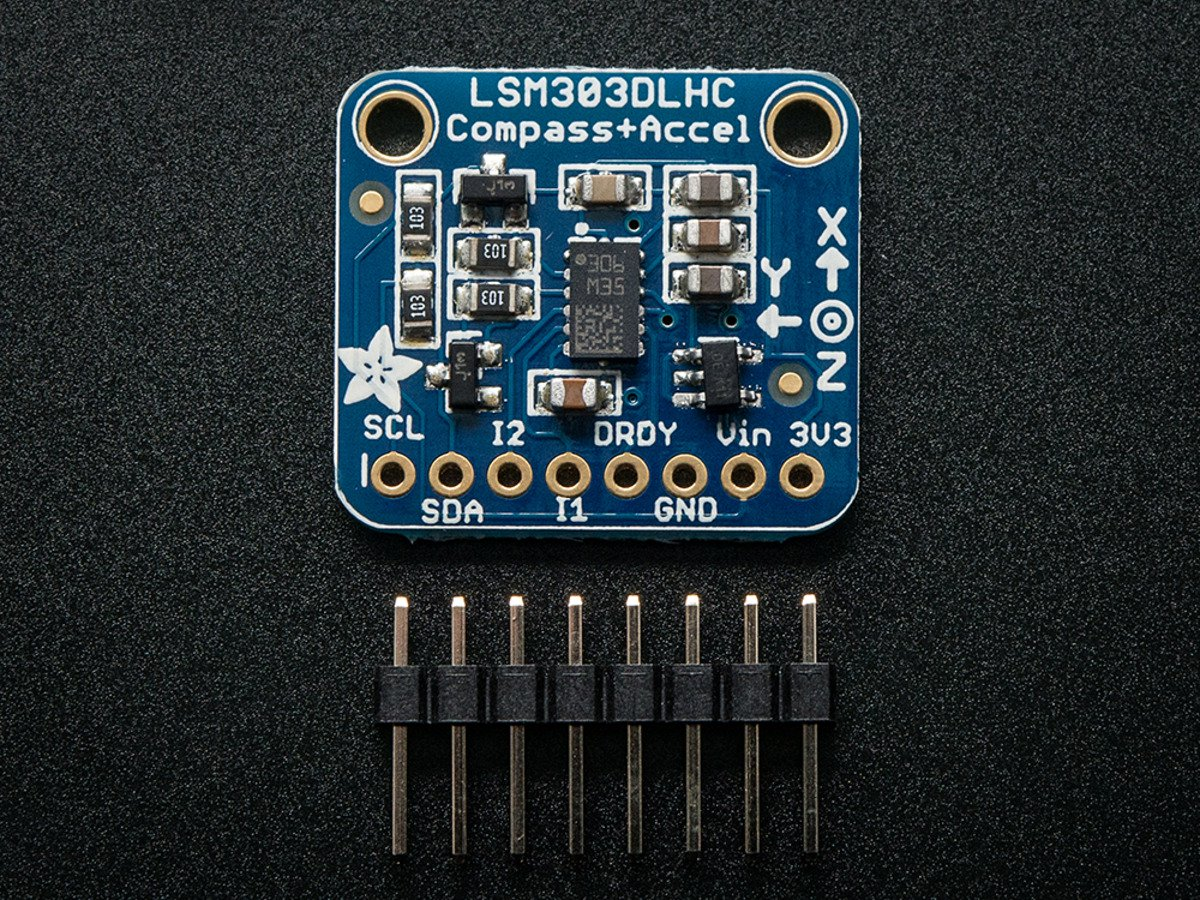
\includegraphics{fig/DOE/LSM}
\caption{LSM303 Triple-axis Accelerometer plus Magnetometer (Compass) Board}
\end{figure}

For the reason of real-time ploting simplicity, the Comma-separated values(CSV) format which provides the timestamp of action, is adopted. The CSV streaming Arduino code\ref{appendix-CSV} is written. The CSV format is like: \textbf{timestamp,sensorName,values,...,checksum}.

For example, one of the result is like this(during around 100ms):

\begin{quote}
\centering
...

33,Acceleration,0.122,-0.022,-8.894,1217

44,Gyro,-0.177,-0.999,-0.142,416

53,Orientation,-179.737,-0.759,7.834,991

64,Acceleration,0.074,-0.062,-8.863,1217

74,Gyro,-0.181,-1.074,-0.112,416

83,Orientation,-179.598,-0.480,7.808,992

95,Acceleration,0.033,-0.067,-8.944,1217

105,Gyro,-0.216,-0.988,-0.177,416

115,Orientation,-179.739,-0.384,7.846,992

126,Acceleration,0.045,-0.010,-8.920,1217

137,Gyro,-0.110,-0.318,-0.061,417

...
\end{quote}

The timestamp is the time value from which the program was runned, in millisecond. The last number is checksum which used for check the communication.
The Baudrate is set as 5700 as softwareSerial does not appear to work reliably above 57600 baud.\cite{https://github.com/ArduSat/ArdusatSDK}
When using Baudrate as 57600, the update frequency of physical quantities are 32Hz, which menas every second we can get 32 groups of acceleration, angular rate and orientation.

\subsection{Xbee modules configuration}
\begin{figure}[!h]
\centering
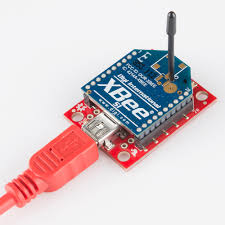
\includegraphics{fig/DOE/XbeeShield}
\caption{Xbee part with Shield}
\end{figure}
Digi XCTU\cite{https://www.digi.com/products/xbee-rf-solutions/xctu-software/xctu} is the software used to configure the Xbee modules. In our case, two Ardusat Demosat should send the real time data to the computers seperately.The two XBee parts are on Ardusat A and Ardusat B The other two Xbee parts are pluged in shields and the shields are connected to Computer A and Computer B respectively. All the Xbee parts should be set carefully\cite{https://learn.sparkfun.com/tutorials/exploring-xbees-and-xctu/configuring-networks}. 
\begin{table}[!h]
\renewcommand\arraystretch{2}
	\begin{center}
	\caption{Xbee parts setting}
	\begin{tabular}{|c|c|c|c|c|}
	\hline
	\backslashbox{\textbf{Setting}}{\textbf{Xbee part}} & \textbf{A shield} & \textbf{On Ardusat A} & \textbf{B shield} & \textbf{On ArduSat B}\\ \hline
	Channel & \multicolumn{2}{c|}{C} &\multicolumn{2}{c|}{17}  \\ \hline
	Personal area network ID & \multicolumn{2}{c|}{3332}& \multicolumn{2}{c|}{83D5}\\ \hline
	Destination Address High & 0 & 0 & 0 & 13A200\\ \hline
	Destination Address Low & 35 & 0 & 1234&4163E25D\\ \hline
	16-bit Source Address & 0 & 35 & 4321 & 1532\\ \hline
	Serial Number High & \multicolumn{4}{c|}{13A200}\\ \hline
	Serial Number Low & 4167BD1E & 4163E2BA & 4163E25D & 4167BD2E\\ \hline
	Interface Data Rate	 & \multicolumn{4}{c|}{57600}\\ \hline
	\end{tabular}	
	\end{center}
\end{table}
The channel controls the frequency band that Xbee commmunicates over. XBee's operate on the 2.4GHZ 802.15.4 band, and the channel further calibrates the operating frequency within that band. The two XBee modules having on the same network operates on the same channel. The two networks are using different channels in case they interatct with each other.

Personal area network ID (PAN ID) is some hexadecimal value between 0 and 0xFFFF. Similar to the channel, the two Xbee modules in the same network must have the same network ID and the different network should have different PAN ID.

 Each XBee in a network should be assigned a 16-bit address (again between 0 and 0xFFFF), which is referred to as MY address, or the “source” address. Another setting, the destination address, determines which source address an XBee can send data to. For one XBee to be able to send data to another, it must have the same destination address as the other XBee's source.

Each XBee has a unique 16-bit Source Address i.e. MY address.

In our case, the task is that On Ardusat A XBee should only send data to to A shield Xbee and On Ardusat B Xbee should only send data to B shield Xbee.

There are two way to configure destination address
\begin{enumerate}
\item Leave Destination Address High set to 0, and set Destination Address Low to the MY address of the receiving XBee.

\item Set Destination Address High to the Serial Number High (SH) and Destination Address Low to the Serial Number Low (SL) of your destination XBee.
\end{enumerate}
To assure that each network has high fidelity and the communication interference between A network and B network is as low as possible, the A network is only using method 1 and the B network is using method 2. A network's configuration obeys method 1 and disobey method 2. B network's configuration obeys method 2 and goes against method 1.

The key is to reduce communication interference when two satellites are moving especially when they are quite close.

\begin{figure}[ht]
\centering
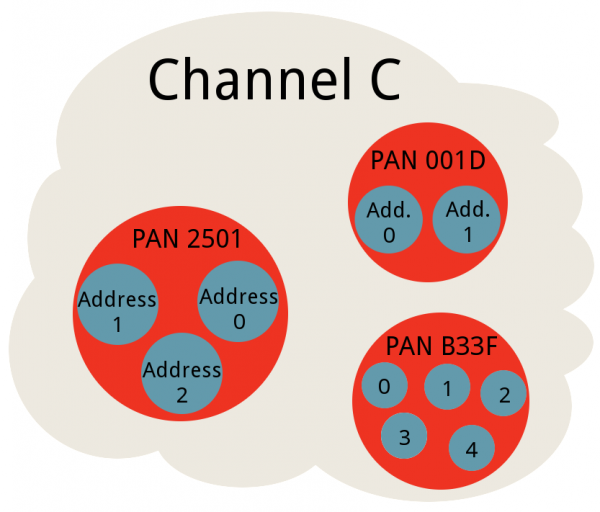
\includegraphics[width=0.5\textwidth]{fig/DOE/Network}
\caption{Xbee-networks}
\end{figure}

\newpage